\documentclass{beamer}
\usepackage{tikz}
\usepackage{pgfplots}
\usepackage{graphicx}
\usepackage{tabu}
\usepackage{booktabs}
\usepackage{fontawesome}
\usepackage{listings}
\usetikzlibrary{positioning}
\usetikzlibrary{calc}
%\usetikzlibrary{arrows}

\usefonttheme{professionalfonts}
\usetheme{Boadilla}
\setbeamertemplate{navigation symbols}{}%remove navigation symbols
\hypersetup{pdfstartview={Fit}} % fits the presentation to the window when first displayed
\graphicspath{{./figures/}{./figures/generated/}{./figures/static/}}
\definecolor{gold}{rgb}{1,.776,.153}
\definecolor{maroon}{rgb}{.549,.114,.251}


%Info
\title[Intro Bioinformatics]{A short introduction to bioinformatics and variant calling}
% \titlegraphic{
	% \includegraphics[width=.3\linewidth]{gatk_tree_rightwards.pdf}
	% \includegraphics[width=.3\textwidth, angle=90]{labeled_tree.jpg}
	% }
\date{5/17/19}
\author{Adam Orr\hskip 1em \faicon{twitter}@AdamJOrr}

\begin{document}
\frame{\titlepage}

\begin{frame}{Outline}
	\begin{itemize}
		\item Sequencing methods and their advantages
		\item FASTQ Format
		\item Read Mapping / Alignment
		\item BAM Format
		\item Variant Calling
		\item VCF Format
		\item Annotation Formats
		\item Assembly?
	\end{itemize}
\end{frame}

\begin{frame}{Sequencing}

	\begin{block}{The Driving Principle}
	We cannot sequence an entire genome or even an entire chromosome accurately in 1 attempt. To sequence we must shred the DNA and sequence the fragments.
	\end{block}

	There are 3 competing sequencing platform providers: Illumina, PacBio, and Oxford Nanopore

	Each platform is based on a different technology that changes how the DNA samples are processed and how sequence information is extracted from them.
\end{frame}

\begin{frame}{Illumina}
	\begin{itemize}
		\item Cheapest and highest throughput
		\item Best single-base accuracy
		\item Reads are short (150 bp)
	\end{itemize}
\end{frame}

\begin{frame}{PacBio SMRT sequencing}
	\begin{itemize}
		\item More expensive but longer reads (10KB)
		\item Decently accurate
		\item Use for long insertions/deletions
	\end{itemize}
\end{frame}

\begin{frame}{Oxford Nanopore: MinION}
	\begin{itemize}
		\item Machine is much more affordable, throughput is lower.
		\item Lowest accuracy, but improving quickly
		\item Longest reads (100KB+)
		\item Use for long insertions/deletions
	\end{itemize}
\end{frame}

\begin{frame}{Sequencing Strategies}
	The less you sequence the less it costs
	\begin{itemize}
		\item Sequencing costs
		\item Data storage costs
		\item Computation costs
	\end{itemize}
	\hskip 1em
	\begin{itemize}
		\item Whole Genome Sequencing
		\item Whole Exome Sequencing
		\item Amplicon Sequencing
	\end{itemize}
\end{frame}

\begin{frame}{Generic Sequencing Experiment Workflow}
	\begin{itemize}
		\item GrCH38 is the current reference
	\end{itemize}
	\vfill
	\begin{centering}
		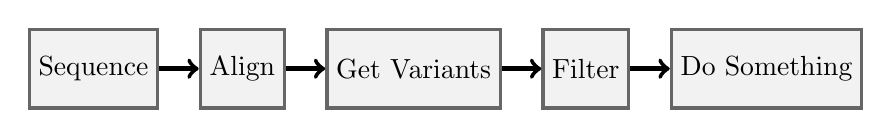
\begin{tikzpicture}[sqnode/.style={rectangle, draw=black!60, fill=black!5,very thick,minimum size=1cm}, node distance = .5cm, align = center]
			\node[sqnode] (sequencing) {Sequence};
			\node[sqnode] (alignment) [right= of sequencing] {Align};
			\node[sqnode] (varcall) [right= of alignment] {Get Variants};
			\node[sqnode] (flt) [right= of varcall] {Filter};
			\node[sqnode] (do) [right= of flt] {Do Something};
			\draw[ultra thick,->] (sequencing.east) -- (alignment.west);
			\draw[ultra thick,->] (alignment.east) -- (varcall.west);
			\draw[ultra thick,->] (varcall.east) -- (flt.west);
			\draw[ultra thick,->] (flt.east) -- (do.west);
		\end{tikzpicture}
	\end{centering}
\end{frame}

\begin{frame}[fragile]{FASTQ Format}
	\begin{itemize}
		\item 4 line format
		\item Most tools transparently work with \texttt{.gz} compressed files.
		\item Quality scores are phred-scaled and encoded as the ASCII value -33. (\texttt{!} = 0, \texttt{J} = 41)
		\item Best resource: wikipedia article on FASTQ format
	\end{itemize}
		\begin{columns}
		\column{.9\linewidth}
		\begin{lstlisting}[frame = single, numbers = left]
@HJCMTCCXX160113:5:1101:1631:47668/1
GCCCAGCACAGAGGTGCCCAGGGTGCAGGCTGGCACTGGC
+
AAFAFF<<<7FFFKFFFFFAAFKAF7FKKKKK(,7A,<KA
		\end{lstlisting}
	\end{columns}
\end{frame}

\begin{frame}{FASTQC}
FASTQC is a quality control program that:
	\begin{itemize}
		\item Checks for adaptor readthrough
		\item Checks there aren't any very obvious biases in the sequenced data
		\item Usually your data will be fine
		\item Ask your sequencing provider what QC they do
		\item Subsamples reads so it's quite fast
	\end{itemize}
\end{frame}

\begin{frame}[fragile]{Read Mapping}
	\begin{itemize}
		\item \texttt{bwa mem} for short reads (GPL3)
		\item \texttt{minimap} for long reads (MIT)
		\item Fairly fast
	\end{itemize}
	\begin{exampleblock}{Algorithm}
	The reference genome is indexed first. The index is used to find plausible locations on the reference for each read, the matches are extended until the most likely location is found.
	\end{exampleblock}
	\begin{lstlisting}[language = bash, frame = single]
bwa index ref.fa
bwa mem reads.1.fq reads.2.fq > aligned.sam
	\end{lstlisting}
\end{frame}

\begin{frame}[fragile]{SAM format}
	\begin{itemize}
		\item Tabular format with header
		\item Binary compressed version called ``\textbf{B}AM".
		\item Highly compressed version called ``\textbf{CR}AM", keep reference handy.
		\item SAMtools is used to view/manipulate BAMs (MIT)
		\item Always sort your bams. MarkDuplicates is a good idea.
		\begin{itemize}
			\item \texttt{samtools sort -Ob aln.sam > aln.sorted.bam}
			\item \texttt{samtools markdup aln.sorted.bam aln.marked.bam}
		\end{itemize}
		\item Resource: The SAM format specification
	\end{itemize}
	\scriptsize{
	\begin{lstlisting}[frame = single]
@HD VN:1.6 SO:coordinate
@SQ SN:ref LN:45
r001   99 ref  7 30 8M2I4M1D3M = 37  39 TTAGATAAAGGATACTG *
r002    0 ref  9 30 3S6M1P1I4M *  0   0 AAAAGATAAGGATA    *
r003    0 ref  9 30 5S6M       *  0   0 GCCTAAGCTAA       * SA:Z:ref,29,-,6H5M,17,0;
r004    0 ref 16 30 6M14N5M    *  0   0 ATAGCTTCAGC       *
r003 2064 ref 29 17 6H5M       *  0   0 TAGGC             * SA:Z:ref,9,+,5S6M,30,1;
r001  147 ref 37 30 9M         =  7 -39 CAGCGGCAT         * NM:i:1
	\end{lstlisting}
	}

\end{frame}

\begin{frame}{Variant Calling}
Mapping is essentially a solved problem; variant calling and subsequent filtering is where things get interesting and start to take a long time.
\vskip 1em
State of the art: local reassembly in regions there may be variation and construct haplotypes.
\vskip 1em
Short variants (substitutions, indels <50bp):
\begin{itemize}
	\item GATK (\$\$\$)
	\item FreeBayes (MIT)
	\item Google DeepVariant (BSD)
\end{itemize}
Long insertions/deletions (>50bp, Structural Variants):
\begin{itemize}
	\item Manta (Illumina; GPL3)
	\item pbsv (PacBio; GPL3)
\end{itemize}
\end{frame}

\begin{frame}[fragile]{VCF Format: Header}
\scriptsize{
\begin{lstlisting}[frame = single, breaklines = true]
##fileformat=VCFv4.3
##fileDate=20090805
##source=myImputationProgramV3.1
##reference=file:///seq/references/1000GenomesPilot-NCBI36.fasta
##contig=<ID=20,length=62435964,assembly=B36,md5=f126cdf8a6e0c7f379d618ff66beb2da,species="Homo sapiens",taxonomy=x>
##phasing=partial
##INFO=<ID=NS,Number=1,Type=Integer,Description="Number of Samples With Data">
##INFO=<ID=DP,Number=1,Type=Integer,Description="Total Depth">
##INFO=<ID=AF,Number=A,Type=Float,Description="Allele Frequency">
##INFO=<ID=AA,Number=1,Type=String,Description="Ancestral Allele">
##INFO=<ID=DB,Number=0,Type=Flag,Description="dbSNP membership, build 129">
##INFO=<ID=H2,Number=0,Type=Flag,Description="HapMap2 membership">
##FILTER=<ID=q10,Description="Quality below 10">
##FILTER=<ID=s50,Description="Less than 50% of samples have data">
##FORMAT=<ID=GT,Number=1,Type=String,Description="Genotype">
##FORMAT=<ID=GQ,Number=1,Type=Integer,Description="Genotype Quality">
##FORMAT=<ID=DP,Number=1,Type=Integer,Description="Read Depth">
##FORMAT=<ID=HQ,Number=2,Type=Integer,Description="Haplotype Quality">
#CHROM POS     ID        REF    ALT     QUAL FILTER INFO                              FORMAT      NA00001        NA00002        NA00003
\end{lstlisting}
}
\end{frame}

\begin{frame}[fragile]{VCF Format: Body}
\scriptsize{
\begin{lstlisting}[frame = single, breaklines = true, keepspaces = false, columns = flexible]
#CHROM POS     ID        REF    ALT     QUAL FILTER INFO                              FORMAT      NA00001        NA00002        NA00003
20     14370   rs6054257 G      A       29   PASS   NS=3;DP=14;AF=0.5;DB;H2           GT:GQ:DP:HQ 0|0:48:1:51,51 1|0:48:8:51,51 1/1:43:5:.,.
20     17330   .         T      A       3    q10    NS=3;DP=11;AF=0.017               GT:GQ:DP:HQ 0|0:49:3:58,50 0|1:3:5:65,3   0/0:41:3
20     1110696 rs6040355 A      G,T     67   PASS   NS=2;DP=10;AF=0.333,0.667;AA=T;DB GT:GQ:DP:HQ 1|2:21:6:23,27 2|1:2:0:18,2   2/2:35:4
20     1230237 .         T      .       47   PASS   NS=3;DP=13;AA=T                   GT:GQ:DP:HQ 0|0:54:7:56,60 0|0:48:4:51,51 0/0:61:2
20     1234567 microsat1 GTC    G,GTCT  50   PASS   NS=3;DP=9;AA=G                    GT:GQ:DP    0/1:35:4       0/2:17:2       1/1:40:3
\end{lstlisting}
}
\end{frame}

\begin{frame}{Variant Filtering}
Tools tend to output many false-positives, so filtering is very important.

\vskip 1em

The variant caller you use will calculate many quality statistics, so exact filters will depend on the method you use and your use case.

\begin{itemize}
	\item BCFTools (MIT or GPL3)
	\begin{itemize}
		\item \texttt{bcftools filter -i 'DP > 10' variants.vcf > variants.filtered.vcf}
	\end{itemize}
	\item Picard (MIT)
	\begin{itemize}
		\item \texttt{java -{}-jar picard.jar FilterVcf INPUT=input.vcf OUTPUT=out.vcf}
	\end{itemize}
	\item VCFTools (GPL3)
	\begin{itemize}
		\item \texttt{vcftools -{}-vcf input.vcf -{}-recode -{}-recode-INFO-all}
	\end{itemize}
\end{itemize}
\end{frame}

\begin{frame}{Annotation Formats}
GFF Format

BED Format

\end{frame}

\end{document}



